\chapter{Обзор платформы Smart-M3}

Smart-M3 --- это открытая программная платформа, воплощающая идеи семантического веба и реализующая инфраструктуру обмена информацией между программными сущностями и устройствами. В данной главе будут рассмотрены технологии, используемые в платформе, архитектура платформы и принципы построения интеллектуальных приложений.

\section{Используемые семантические технологии}


Семантический веб \cite{semantic} -- одно из направлений развития Интернет, целью которого является реализация возможности машинной обработки информации, доступной во Всемирной паутине. Основной акцент концепции делается на работе с метаданными, однозначно характеризующими свойства и содержание ресурсов Всемирной паутины, вместо используемого в настоящее время текстового анализа документов.
Машинная обработка возможна в семантическом вебе благодаря двум характеристикам.

{\bf 1. Использование унифицированных идентификаторов ресурсов (URI)}.
Традиционная схема использования таких идентификаторов в современном Интернете сводится к установке ссылок, ведущих на объект, им адресуемый. Очевидным свойством такой ссылки является возможность «загрузки» объекта, на который она указывает. Таким объектом может быть веб-страница, файл произвольного содержания, фрагмент веб-страницы, а также неявное указание на обращение к реально существующему физическому ресурсу по протоколу, отличному от HTTP (например, ссылки mailto:). Концепция семантической паутины расширяет это понятие, включая в него ресурсы, недоступные для скачивания. Адресуемыми с помощью URI ресурсами могут быть, например, отдельные люди, города и другие сущности.

{\bf 2. Использование онтологий и языков описания метаданных}.
В семантическом вебе предлагается использовать форматы описания, доступные для машинной обработки (например, семейство форматов, часто упоминаемое в литературе как «Semantic Web family»: RDF, RDF Schema или RDF-S, и OWL), в свою очередь, использующие URI для адресации описываемых и описывающих объектов.

На платформе Smart-M3 используется схема описания данных основанная на RDF.
Resource Description Framework (RDF) --- это разработанная консорциумом Всемирной паутины модель для представления данных, в особенности -- метаданных. RDF представляет утверждения о ресурсах в виде, пригодном для машинной обработки. Ресурсом в RDF может быть любая сущность -- как информационная (например, веб-сайт или изображение), так и неинформационная (например, человек, город или некое абстрактное понятие). Утверждение, высказываемое о ресурсе, имеет вид «субъект -- предикат -- объект» и называется {\it триплетом}. Утверждение «небо голубого цвета» в RDF-терминологии можно представить следующим образом: субъект -- «небо», предикат -- «имеет цвет», объект -- «голубой». Для обозначения субъектов, предикатов и объектов в RDF используются URI. Множество RDF-утверждений образует ориентированный граф, в котором вершинами являются субъекты и объекты, а рёбра помечены предикатами.

Также для работы с Smart-M3 можно использовать специальные генераторы. Генератор на основе файла, описанного в формате OWL, создаёт приложение, которое может взаимодействовать с платформой.

OWL --- язык описания онтологий для семантического веба. Язык OWL позволяет описывать классы и отношения между ними, присущие для веб-документов и приложений. OWL основан на более ранних языках OIL и DAML+OIL и в настоящее время является рекомендованным консорциумом Всемирной паутины.

В основе языка --- представление действительности в модели данных «объект — свойство». OWL пригоден для описания не только веб-страниц, но и любых объектов действительности. Каждому элементу описания в этом языке (в том числе свойствам, связывающим объекты) ставится в соответствие URI.

\section{Архитектура платформы Smart-M3}
В мире существуют миллиарды мобильных устройств. Многие из них обладают неплохими размерами памяти и достаточной вычислительной мощностью. Если любые устройства смогут передавать друг другу информацию, то это качественно изменит жизнь людей, повысит уровень автоматизации по всех областях.

Ключевой идеей Smart-M3 является то, что устройства и программные сущности могут обмениваться между собой информацией.
Одни из барьеров во взаимодействии между различными устройствами является разница в форматах информации, которую они распознают и с которой работают. Такие технологии как XML, RDF, OWL обеспечивают методы, позволяющие сфокусироваться на семантике информации а не на её синтаксическом представлении. Организация взаимодействия между устройствами и приложениями, работающими на них, является непростой задачей. Но был выбран прямолинейный подход: есть некоторое количество устройств и <<доска>>, которая может использоваться для обмена информацией между этими устройствами, вместо того, чтобы устройства явно посылали друг другу сообщения. Кроме того, если эта информация будет храниться согласно некоторой онтологии, то станет возможен обмен этой информацией между устройствами, использующими разную модель представления данных, засчёт фокусировки на семантике информации.

M3 расшифровывается как multi-vendor, multi-device and multi-part (много продавцов, много устройств, много частей).
Это означает что множество видов устройств могут взаимодействовать друг с другом, например, мобильный телефон, телевизор и ноутбук. Устройства могут состоять из частей, которые подразумеваются как отдельные участники взаимодействия с другим устройством. Кроме этого пользователь свободен в выборе производителя. Smart-M3 разрабатывается так, чтобы была возможность работы в различных средах, учитывая их ограничения. Технология позволяет создавать программы, которые смогут использовать возможности, предоставляемые окружением устройства.

Подход Smart-M3 отклоняет прямое взаимодействие между устройствами и использует механизм <<публикации и чтения>>. Сущность, предоставляющая информацию не нуждается во взаимодействии с читающей сущностью. Фактически эти две сущности даже могут не знать друг о друге. Smart-M3 предлагает, что публикующая сущность может разместить информацию в спецальном месте обмена информации, а читающая сущность взять её оттуда.

Взаимодействие между сущностями в Smart-M3 можно логически разделить на три уровня:

\begin{itemize}
\item
нижний уровень -- <<мир устройств>>, на нём находится множество устройств, соединённых сетью
\item
средний уровень -- <<мир сервисов>>, на нём находятся программы, клиенты и сервисы. Сервисы доступны только внутри конкретного домена. Обмен информацией осуществляется засчёт специальных протоколов обмена сообщениями
\item
верхний уровень -- <<умный мир>>, в нём взаимодействие основано на семантике информации. <<Умный мир>> унифицирует нижние уровни совместимостью на информационном уровне
\end{itemize}

\begin{figure}[h]
\centerline{
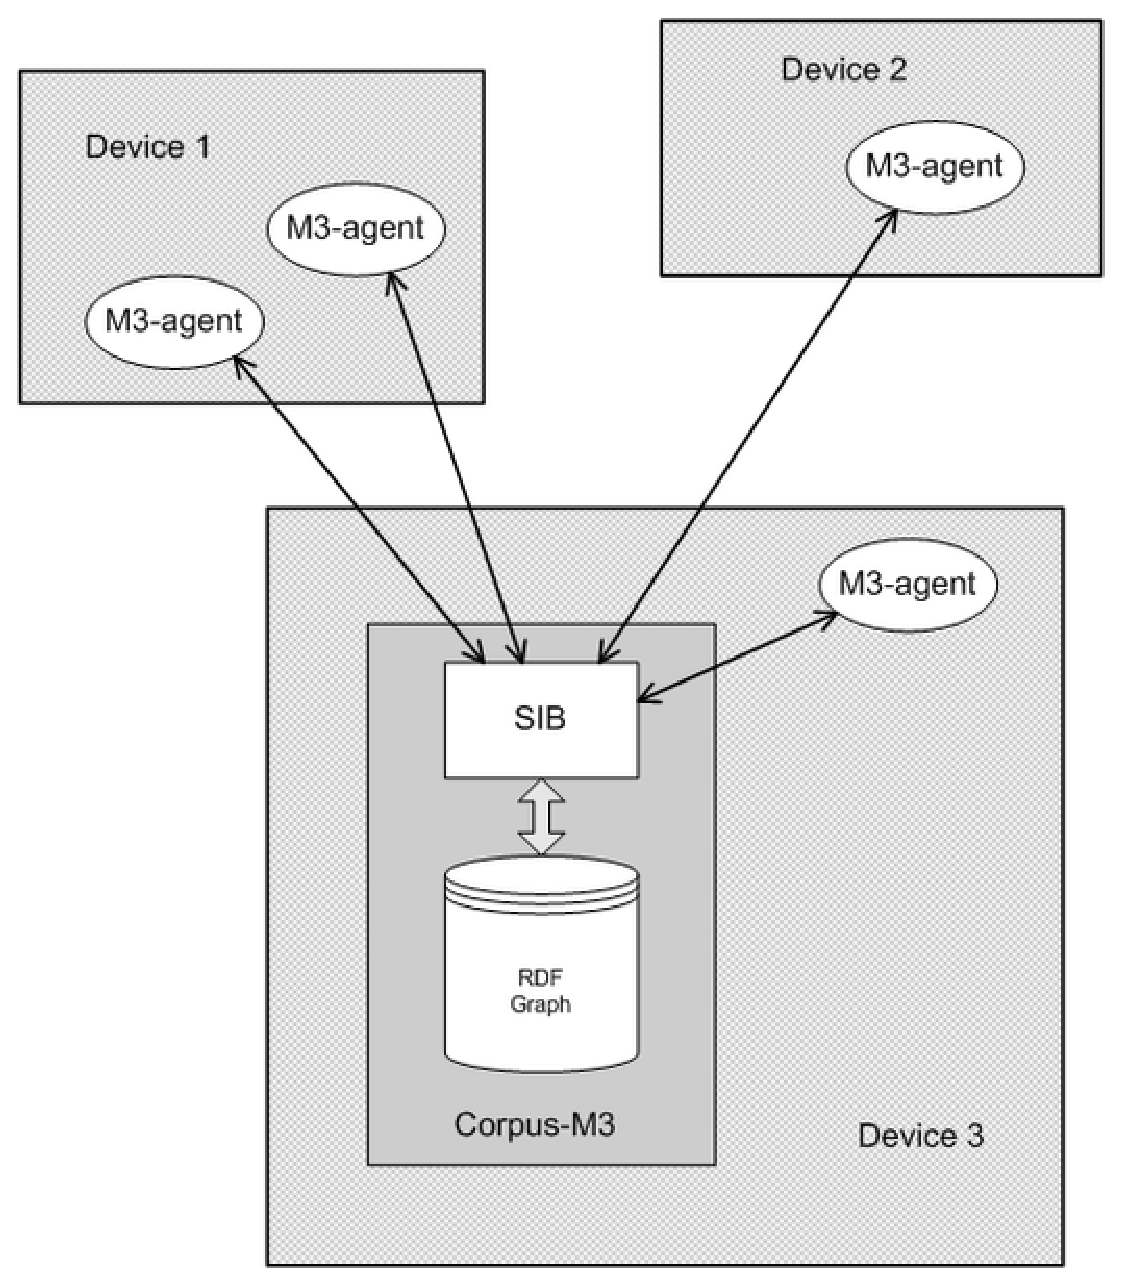
\epsfig{file=images/smartm3.eps, width=10cm}}
\caption{Архитектура Smart-M3}
\label{smart-m3}
\end{figure}
Рассмотрим архитектуру платформы Smart-M3 (рис. \ref{smart-m3}). Центром системы является corpus-M3, который можно разбить на две главные части: брокер семантической информации (semantic information broker, далее SIB) и реальное физическое хранилище данных (БД).

SIB --- это точка доступа для получения или отправки информации в хранилище. Вся информация в хранилище представлена в виде графа, который соответствует правилам RDF.

M3-agent --- это приложение, которое взаимодействует с SIB: публикует или получает отуда информацию. M3-agent может находиться на другом устройстве и взаимодействовать с SIB, используя различные средства связи, поддерживаемые SIB.
SIB может поддерживать множество протоколов передачи данных, таких как TCP/IP, Bluetooth и NoTA. В зависимости от окружения где запущен агент, выбирается более подходящая технология передачи информации.
Конкретный M3-agent связан с конкретным SIB. 

Также M3-agent называют <<процессором знаний>> (knowledge processor, далее KP), так как он обрабатывает информацию и публикует её в SIB или запрашивает её для обработки.

KP состоит из пользовательского интерфейса, логики обработки данных и <<узла>> (node). SmartSpace состоит из SIB и хранилища информации. На одном устройстве может работать множество KP. Пользовательский интерфейс для KP может быть не важен и представлять собой, например LCD дисплей или кнопку. <<Узел>> -- это часть KP, которая содержит всю логику и функциональность для связи KP с некоторым SmartSpace (SIB): логика обработки сообщений и обработчики подписки между KP и SIB. KP может содержать множество <<узлов>> и тем самым быть соединённым с несколькими SIB.

Идея Smart-M3 приводит к новому взгляду на разработку приложений. Приложение не является монолитным, а состоит из несколько частей --- KP, которые взаимодействуют между собой через SIB. Количество агентов может быть различным в зависимости от конкретной ситуации и требований пользователя. 

Взаимодействие между агентом и SIB осуществляется через протокол доступа к ИП (Smart Space Access Protocol, SSAP). Основные операции SSAP:
\begin{itemize}
\item
Join -- соединить KP с указанным пространство
\item
Leave -- покинуть ИП\\
После выполнения данной операции, другие операции не могут быть выполнены до повторного соединения с ИП.
\item
Insert -- атомарно разместить информацию (RDF-граф) в ИП
\item
Remove -- атомарно удалить информацию
\item
Update -- атомарно обновить информацию\\
Обновление является комбинацией операций удаления и добавления, но выполняется атомарно.
\item
Query -- запросить информацию из ИП, используя поддерживаемый язык запросов
\item
Subscribe -- подписаться на некоторую информацию и получать все её изменения
\item
Unsubscribe -- отмена существующей подписки
\end{itemize}
Протокол SSAP гарантирует, что все операции будут выполнены в том порядке, в котором они были вызваны в агенте.

\section{Понятие Smart-M3 приложения}

Для интеллектуальных приложений необоходимо проектировать сценарии, подразумевающие, что каждый из KP может быть запущен на различных устройствах. Каждый агент, выполняя некоторые действия, представляет собой сервис. Взаимодействие между KP можно рассматривать с двух точек зрения: с точки зрения использования сервисов и изменения данных в ИП. При выполнении операций join и leave агент соединяется или отсоединяется от ИП, а сервис, который он предоставляет, становится доступным/недоступным. При взаимодействии между собой агенты запрашивают и модифицируют данные из ИП. Несмотря на использование механизма публикации-подписки агенты могут взаимодействовать между собой и напрямую по сети, однако данный вид взаимодействия не относится к концепции ИП.

Каждый агент имеет представление о собственном наборе информации, являющейся частью глобального RDF-графа в ИП. Такие знания описываются 
онтологией агента. Для осуществления взаимодействия между агентами, необходимо наличие пересечения между онтологиями каждого из них. Таким образом в местах пересечения агенты могут отслеживать действия друг друга.

Все агенты можно разделить на три класса по характеру работы с данными: агенты-поставщики (только публикуют новые данные), агенты-потребители (только читают необходимые данные) и агенты, которые обрабатывают полученные данные и на их основе производят и публикуют новые знания.

На данный момент в платформе Smart-M3 существует несколько открытых проблем. Одна из них связана с ситуацией конкуренции между агентами за одни и те же ресурсы. Вследствие осутствия механизма синхронизации, результат такого взаимодействия неопределён.

Другой задачей является осуществление взаимодействия между агентами из разных приложений. Такие агенты обладают разными онтологиями и для решения данной проблемы необходима разработка методов осуществления композиции или пересечения онтологий. Таким образом для комбинации интеллектуальных приложений необходимо пересечение их ИП, которое может быть осуществлено благодаря пересечению онтологических знаний. В таких приложениях будут появляется агенты-посредники, взаимодействующие с несколькими пространствами. Подробнее эта проблема рассматривается в главе 3.

Агенты взаимодействуют с SIB по протоколу SSAP через библиотеки, предоставляющие интерфейс процессора знаний (KP interface, KPI). Большинство таких библиотек предоставляет функции, выполняющие прямой доступ к протоколу SSAP. Соответственно работа агента с онтологическими данными заключается в обмене обработке триплетов. Такой подход является низкоуровневым.

Существует также высокоуровневый подход к осуществлению взаимодействия с онтологическими данными. В таком случае работа происходит с более общими сущностями вместо триплетов. Данный подход предусматривает наличие генератора, создающего библиотеку, основанную на онтологических сущностях \cite{korzun:smartslog}. Высокоуровневое взаимодействие позволяет разработчику работать с данными в терминах классов и их свойств.

В проекте SmartScribo, который будет рассмотрен в главе 2, использовалась низкоуровневая библиотека M3-Python KPI (m3\_kp). Данная библиотека позволяет реализовывать интеллектуальные агенты на языке Python. В проекте использовалась библиотека m3\_kp вследствие того, что она позволяет более простым способом организовывать взаимодействие с SIB, а также на языке Python намного проще выполнять другие операции приложения SmartScribo. Особенностью библиотеки m3\_kp является выполнение каждой подписки в отдельном потоке, в отличие от библиотек, использующих языки C/C++, где выполнение подписки в потоке программисту приходится реализовывать самому.

Платформа Smart-M3 обладает широкими возможностями для разработки распределённых приложений и, в отличии от традиционного подхода к реализации приложения, позволяет расширять возможности программ, засчёт кооперации между различными интеллектуальными агентами и онтологического представления информации.

